\section{Simulation Analysis}
\label{sec:simulation}

\subsection{Audio Amplifier Simulation}
\label{subsec:amp_simulation}
\par In this section we simulate a BPF using the NGspice tool. Our goal is to simulate the circuit to obtain the output voltage gain, the central frequency, and both the input and output frequencies at the specified central frequency (1kHz).

\par  \textbf{Important note:} Beyond modelling and analysing the circuit provided, one of the goals of this laboratory assignment is to maximize the merit, which is computed according to the following formula:
\begin{equation}
M = \frac{1}{\text{cost}*(\text{Voltage Gain Deviation}+\text{Central Frequency Deviation}+10^{-6})}
\label{eq:merit}
\end{equation}

\par Therefore, it was our intention to obtain the best value for this parameter,using each of the variables in order to maximize it, wich means that we have not tried to improve each of those separately, but as a all. This value is presented in Subsection \ref{merit}.
In order to do it we used the values indicated the following values of the components: $R_{11}=1k\Omega$, $R_{12}=1k\Omega$, $R_{2}=1k\Omega$, $R_{31}=100k\Omega$, $R_{32}=100k\Omega$, $R_{33}=100k\Omega$, $R_{41}=10k\Omega$, $R_{42}=10k\Omega$, $C_{1}=220nF$, $C_{21}=220nF$ and $C_{22}=220nF$. 

\par Notice that in order to simplify the circuit the equivalent resistors and capacitors were considered in the simulation.
\begin{itemize}
\item $R_{1} = 2 \times 1k_{ R} (parallel)$
\item $R_{3} = 3 \times 100k_{ R} (series)$
\item $R_{4} = 2 \times 10k_{ R} (parallel)$
\item $C_{2} = 2 \times 220n_{ R} (series)$
\end{itemize}

The cost of these components can be computed according to the values provided in the slides, wich leads to the following total cost:

\begin{table}[H]
  \centering
  \begin{tabular}{ |l|r| } 
    \hline    
    {\bf Cost} & {\bf Value} \\ \hline
    \input{../sim/cost_tab}
  \end{tabular}
  \caption{Cost}
  \label{tab:cost}
\end{table}


\subsection{Output Voltage Gain}
\label{output_gain}
\par In order to compute the output voltage gain, we used Ngspice's \textit{abs} function to determine the the magnitude coefficient between the output voltage $v(out)$ and the input voltage $v(in)$ at point $[20]$.

 \par In the following table, we present the magnitude of the gain, in both linear units and decibels as well as its deviation from the specified value (40db or 100 [Linear]) in the same units.
 Note that a gain of $40dB$ in decibels corresponds to a gain of $10^{\frac{40}{20}}=10^2=100$ in linear units.
 The absolute gain deviation was computed in linear units and decibels from $gain_dev_lin= abs(gain-100)$ and $gain_dev_db = abs(gaindb-40)$, respectively. 
 
\begin{table}[H]
  \centering
  \begin{tabular}{|l|r|}
    \hline    
    {\bf Output Voltage Gain} & {\bf Value} \\ \hline
    Output Voltage Gain dB & 266.369\\ \hline
Central Freq & 949.276\\ \hline
Low CO Freq & 453.95\\ \hline
Up CO Freq & 1985.08\\ \hline
Gain Deviation & 166.369\\ \hline
Gain Deviation dB & 8.50966\\ \hline
Central Freq Deviation &50.724\\ \hline
Bandwidth & 1531.13\\ \hline

  \end{tabular}
  \caption{Output Voltage Gain and Deviation, in Linear Units and dB}
  \label{tab:gain}
\end{table}

\par Beyond the magnitude, one can represent the phase of the output voltage, as shown in the following figure:

\begin{figure}[H] \centering
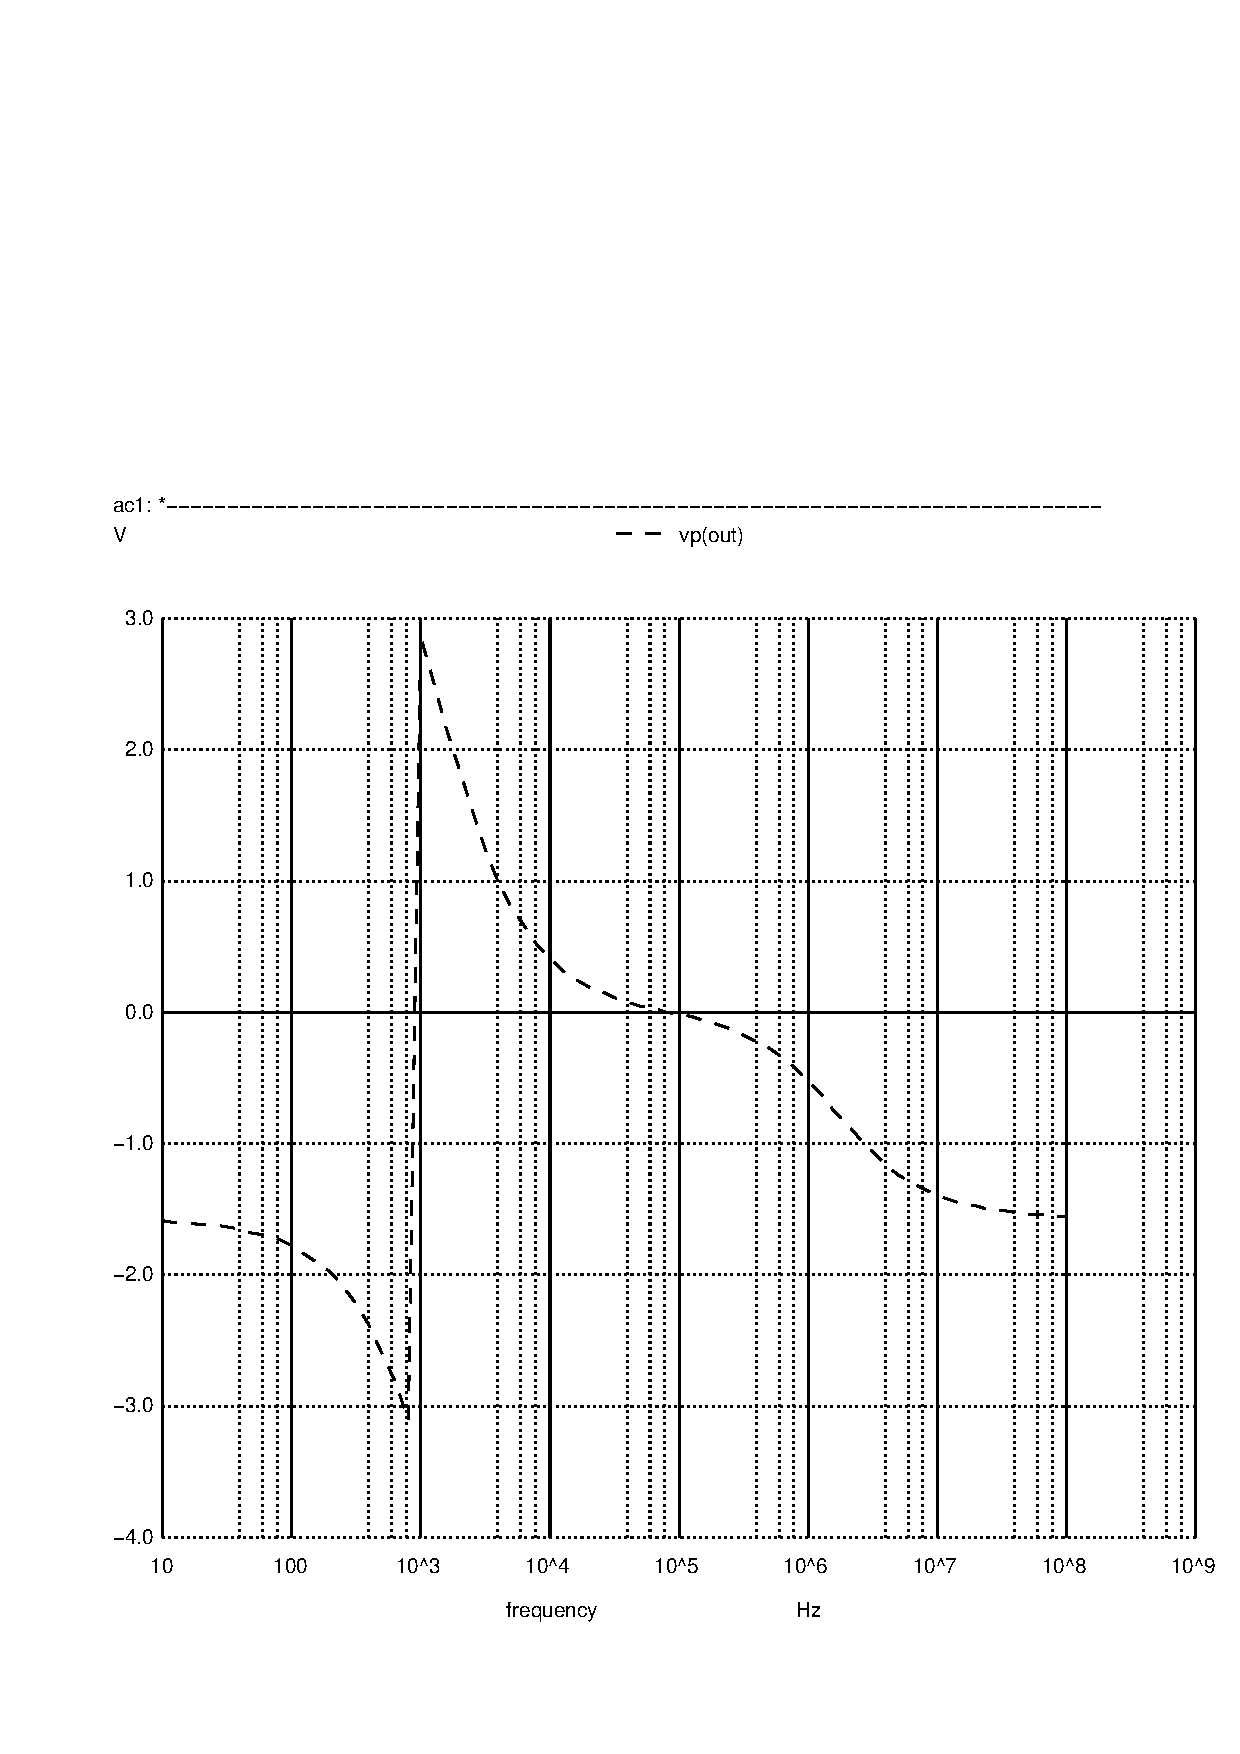
\includegraphics[clip, trim=1.3cm 1.3cm 0cm 7cm, width=0.6\linewidth]{vp.pdf}
\caption{Output Voltage Phase, in Degrees}
\label{fig:vp}
\end{figure}



\subsection{Frequency Response - Central Frequency}
\label{frequency_response}
\par In this subsection, we use the Ngspice's \textit{measure} function to compute the value of the lower and upper 3db cut off frequencies, which allowed the calculation of the central frequency. Beyond this, it is also presented the bandwidth which is the difference between the lower and upper cut off frequencies.
\par The lower and upper frequencies are the frequencies to which the output voltage gain is 3 dB lower than the maximum gain. We can determine this values using the \textit{measure} function. Once we get the lower and upper cutoff frequencies we can determine the central frequency using the geometric average given by $f_{central}=\sqrt{f_{lower}\times f_{upper}}$ and the bandwidth subtracting the lower cutoff frequency from the upper cutoff frequency: $Bandwidth = f_{upper}-f_{lower}$.
The values for these frequencies and the computed bandwidth are presented bellow:

\begin{table}[H]
  \centering
  \begin{tabular}{|l|r|}
    \hline    
    {\bf Variable} & {\bf Value [Hz]} \\ \hline
    \input{../sim/freq_tab}
  \end{tabular}
  \caption{Lower and Upper Cut off Frequencies, Central Frequency and Bandwidth, in Hz}
  \label{tab:frequencies}
\end{table}

\par In the following plot, one can observe both the gain described in the previous section as well as the central frequency of the output voltage:
\begin{figure}[H] \centering
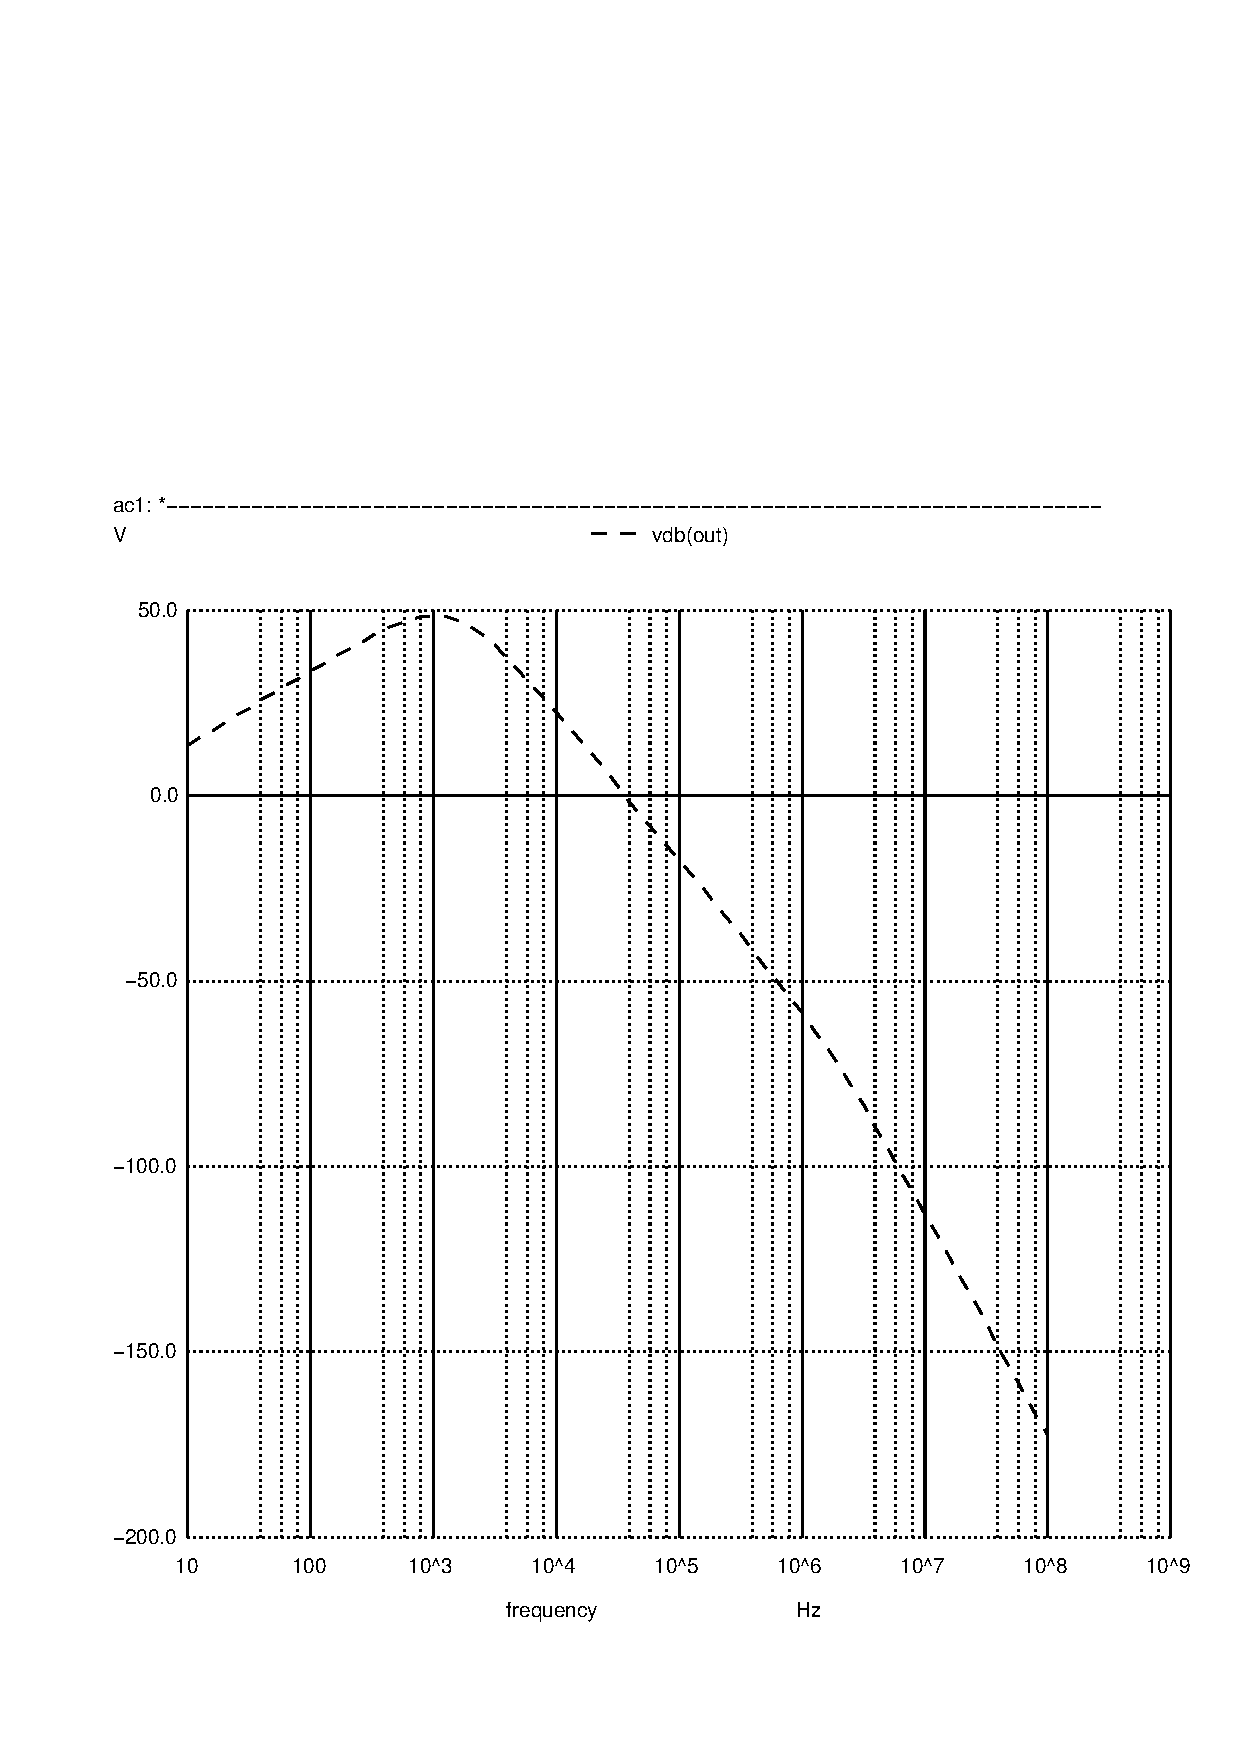
\includegraphics[clip, trim=1.3cm 1.3cm 0cm 7cm, width=0.6\linewidth]{vdb.pdf}
\caption{Output Voltage, in dB}
\label{fig:vdb}
\end{figure}

Now, one can compute the central frequency deviation from the specified value of 1kHz ($f_{deviation}=abs[f_c-1000]$):

\begin{table}[H]
  \centering
  \begin{tabular}{|l|r|}
    \hline    
    {\bf Variable} & {\bf Value [Hz]} \\ \hline
    \input{../sim/freq_dev_tab}
  \end{tabular}
  \caption{Central Frequency Deviation, in Hz}
  \label{tab:frequency_dev}
\end{table}


\subsection{Impedances}
\label{impedances}
\par Finally, in this subsection the input impedance and the output impedance are presented.
\par The input impedance is given by the coefficient between the voltage and the current in the input branch at poin [20]. On the other hand, to compute the output impedance the input voltage source was removed and was added a test voltage source. The output impedance is so given by the coefficient between the voltage and the current in the test voltage source $VL$ branch. The results obtained are shown in the following tables:

\begin{table}[H]
  \centering
  \begin{tabular}{|l|r|}
    \hline    
    {\bf Input Impedance} & {\bf Value [S]} \\ \hline
    zi & 5.638527e-01,-8.44302e-02\\ \hline

  \end{tabular}
  \caption{Input Impedance, in Siemens}
  \label{tab:input_z}
\end{table}


\begin{table}[H]
  \centering
  \begin{tabular}{|l|r|}
    \hline    
    {\bf Output Impedance} & {\bf Value [S]} \\ \hline
    zo & -1.00554e+01,1.184265e+00\\ \hline

  \end{tabular}
  \caption{Output Impedance, in Siemens}
  \label{tab:output_z}
\end{table}





\subsection{Merit}
\label{merit}

\par Recalling the equation \ref{eq:merit} in the Subsection \ref{sec:simulation}, one can notice that the merit depends on three variables computed in previous sections.
\par The components and the layout explained above led to the following merit value:

\begin{table}[H]
  \centering
  \begin{tabular}{ |l|r| } 
    \hline    
    {\bf Merit} & {\bf Value} \\ \hline
    Merit & 1.75991E-10\\ \hline
Cost & 673324 MU\\ \hline

  \end{tabular}
  \caption{Merit Calculation}
  \label{tab:merit}
\end{table}

\par The cost of the components used in the circuit analysed was presented in Subsection \ref{sec:simulation}.
\par Regarding the gain deviation, the considered value was the one in linear units.
\par The central frequency deviation used in the merit formula was the one obtained in Subsection \ref{frequency_response}.
